\documentclass{book}

\usepackage{amsmath, amsthm, amssymb, amsfonts}
\usepackage{thmtools}
\usepackage{graphicx}
\usepackage{setspace}
\usepackage{geometry}
\usepackage{float}
\usepackage{hyperref}
\usepackage[utf8]{inputenc}
\usepackage[french]{babel}
\usepackage{framed}
\usepackage[dvipsnames]{xcolor}
\usepackage{tcolorbox}

\usepackage{algorithm}
\usepackage[noend]{algpseudocode}
\usepackage{etoolbox}

\usepackage{algpseudocode}

\usepackage[table]{xcolor}
\usepackage{colortbl}

\usepackage{stmaryrd}

\usepackage{listings}
\usepackage{xcolor} % Pour personnaliser les couleurs (optionnel)

\lstset{
  language=Python,                % Spécifie le langage (ici Python)
  basicstyle=\ttfamily\small,     % Style de base (taille et police)
  keywordstyle=\color{blue},      % Couleur des mots-clés
  stringstyle=\color{red},        % Couleur des chaînes de caractères
  commentstyle=\color{gray},      % Couleur des commentaires
  numbers=left,                   % Numérotation des lignes (à gauche)
  numberstyle=\tiny\color{gray},  % Style des numéros de ligne
  stepnumber=1,                   % Numérotation toutes les lignes
  breaklines=true,                % Retour à la ligne automatique
  frame=single,                   % Encadrer le code
  captionpos=b                    % Position de la légende (en bas)
}


\colorlet{LightGray}{White!90!Periwinkle}
\colorlet{LightOrange}{Orange!15}
\colorlet{LightGreen}{Green!15}

\newcommand{\HRule}[1]{\rule{\linewidth}{#1}}

\newcommand{\Lcell}{\cellcolor{blue!50}\color{white}L}
\newcommand{\Ccell}{\cellcolor{red!50}\color{white}C}
\newcommand{\Zcell}{\cellcolor{yellow!50}0}


\declaretheoremstyle[name=Theoreme,]{thmsty}
\declaretheorem[style=thmsty,numberwithin=section]{theorem}
\tcolorboxenvironment{theorem}{colback=LightGray}

\declaretheoremstyle[name=Proposition,]{prosty}
\declaretheorem[style=prosty,numberlike=theorem]{proposition}
\tcolorboxenvironment{proposition}{colback=LightOrange}

\declaretheoremstyle[name=Definition,]{prcpsty}
\declaretheorem[style=prcpsty,numberlike=theorem]{principle}
\tcolorboxenvironment{principle}{colback=LightGreen}

\setstretch{1}
\geometry{
    textheight=9in,
    textwidth=5.5in,
    top=1in,
    headheight=12pt,
    headsep=25pt,
    footskip=30pt
}


\begin{document}

\begin{titlepage}

    
\includegraphics[width=8cm]{photo.png} \hfill
    
\includegraphics[width=3cm]{logo.png}

    \vspace{4cm}

    \begin{center}
        \HRule{1.5pt} \\[0.4cm]
        {\LARGE \textbf{\uppercase{TP Apprentissage statistique}}} \\[0.4cm]
        \HRule{2pt} \\[0.6cm]
        {\Large Compte rendu} \\[6cm]



        \textbf{Kilian Saint-Chely} \\[0.5cm]
        Professeur : Bilel Bensaid \\[0.3cm]
        Master Statistiques et Science des Données \\[0.3cm]
        Université de Montpellier \\[2cm]

        {\large 3 octobre 2025}
    \end{center}
\end{titlepage}
\tableofcontents
\newpage

% ------------------------------------------------------------------------------

\chapter{Classification des iris}

\section{Importation des librairies et préparation des données}

Avant de commencer, nous importons les librairies et le jeu de données nécessaire au TP

\begin{lstlisting}[language=Python, caption=Préparation]
import numpy as np
import matplotlib.pyplot as plt
from sklearn.svm import SVC

from svm_source import *
from sklearn import svm
from sklearn import datasets
from sklearn.utils import shuffle
from sklearn.preprocessing import StandardScaler
from sklearn.model_selection import train_test_split, GridSearchCV
from sklearn.datasets import fetch_lfw_people
from sklearn.decomposition import PCA
from time import time

scaler = StandardScaler()

import warnings
warnings.filterwarnings("ignore")

plt.style.use('ggplot')

iris = datasets.load_iris()
X = iris.data
X = scaler.fit_transform(X)
y = iris.target
X = X[y != 0, :2]
y = y[y != 0]
\end{lstlisting}

Ensuite nous séparons les données dans l'optique de réaliser une validation croisée. On garde 25\% de nos données pour le test et 75\% pour l'apprentissage. Enfin, nous fixons une graine pour la reproductibilité du TP.

\begin{lstlisting}[language=Python, caption=Séparation pour validation croisée]
X_train, X_test, y_train, y_test = train_test_split(X, y, test_size=0.25, random_state=42, shuffle=True)
\end{lstlisting}

\section{Classification à partir d'un noyau linéaire}

Dans cette section, nous mettons en place un code qui va classifier la classe 1 contre la classe 2 à l'aide d'un noyau linéaire. Nous regardons alors le meilleur paramètre C et les scores sur les données d'entraînement et de tests.

\begin{lstlisting}[language=Python, caption=Classification des classes 1 contre 2 avec noyau linéaire]
# fit the model and select the best hyperparameter C
parameters = {'kernel': ['linear'], 'C': list(np.logspace(-3, 3, 200))}
clf_linear = GridSearchCV(SVC(), parameters, n_jobs=-1)
clf_linear.fit(X_train, y_train)

# compute the score
print(clf_linear.best_params_)
print('Generalization score for linear kernel: %s, %s' %
      (clf_linear.score(X_train, y_train),
       clf_linear.score(X_test, y_test)))
\end{lstlisting}

Les observations que l'on peut faire sont les suivantes:\\ 
- le meilleur paramètre est C=0.84\\
- le score du jeu d'entraînement est 0.75 \\
- le score sur l'ensemble test est 0.68 ($<$0.75, ce qui est logique puisqu'un modèle colle toujours mieux aux données d'entraînement) 

\section{Classification à partir d'un noyau polynomial}

Nous effectuons à présent la même classification mais avec un noyau polynomial où on teste les degrés 1, 2 et 3. 

\begin{lstlisting}[language=Python, caption=Classification des classes 1 contre 2 avec noyau polynomial]
Cs = list(np.logspace(-3, 3, 5))
gammas = 10. ** np.arange(1, 2)
degrees = np.r_[1, 2, 3]

# fit the model and select the best set of hyperparameters
parameters = {'kernel': ['poly'], 'C': Cs, 'gamma': gammas, 'degree': degrees}

clf_poly = GridSearchCV(SVC(), parameters, n_jobs=-1)
clf_poly.fit(X_train, y_train)

print(clf_poly.best_params_)
print('Generalization score for polynomial kernel: %s, %s' %
      (clf_poly.score(X_train, y_train),
       clf_poly.score(X_test, y_test)))
\end{lstlisting}

Il ressort de ce test, que le noyau polynomial le plus performant est celui de degré 1; avec exactement le même score que le noyau linéaire. Ceci est cohérent puisque le degré d'un noyau linéaire est 1. 

\section{Visualisation de nos classifications}

On écrit un code permettant de visualiser les données et les frontières que nous avons tracées.

\begin{lstlisting}[language=Python, caption=Visualisation des données et des classifications]
# display your results using frontiere (svm_source.py)

def f_linear(xx):
    return clf_linear.predict(xx.reshape(1, -1))

def f_poly(xx):
    return clf_poly.predict(xx.reshape(1, -1))

plt.ion()
plt.figure(figsize=(15, 5))
plt.subplot(131)
plot_2d(X, y)
plt.title("iris dataset")

plt.subplot(132)
frontiere(f_linear, X, y)
plt.title("linear kernel")

plt.subplot(133)
frontiere(f_poly, X, y)
plt.title("polynomial kernel")

plt.tight_layout()
plt.draw()
\end{lstlisting}

On peut constater sur la figure 1.1 que la frontière est sensiblement différente malgré un score de performance identique. Cela s'explique par le fait que le noyau linéaire est sans terme de biais, alors que le noyau polynomial de degré 1 est une forme affine (avec biais). 

\begin{figure}[H] % [H] = force l'image à rester ici
    \centering
    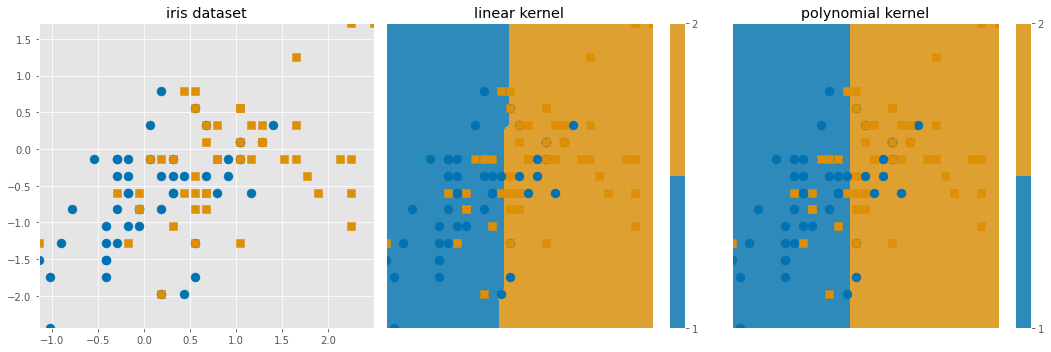
\includegraphics[width=1\textwidth]{figure 1.png}
    \caption{Visualisation des données et des frontières}
    \label{fig:exemple}
\end{figure}

\section{Reprise d'un noyau polynomial en retirant le degré 1}

Dans cette partie, nous reprenons le même procédé que les deux sections précédentes, mais en retirant la possibilité de degré 1 pour le noyau polynomial afin de visualiser ce que cela donnerait comme résultat.

\begin{lstlisting}[language=Python, caption=Programme de classification et de visualisation avec un noyau polynomial de degré supérieur à 1]
Cs = list(np.logspace(-3, 3, 5))
gammas = 10. ** np.arange(1, 2)
degrees = np.r_[2, 3]

# fit the model and select the best set of hyperparameters
parameters = {'kernel': ['poly'], 'C': Cs, 'gamma': gammas, 'degree': degrees}

clf_poly2 = GridSearchCV(SVC(), parameters, n_jobs=-1)
clf_poly2.fit(X_train, y_train)

print(clf_poly2.best_params_)
print('Generalization score for polynomial kernel: %s, %s' %
      (clf_poly2.score(X_train, y_train),
       clf_poly2.score(X_test, y_test)))

def f_poly2(xx):
    return clf_poly2.predict(xx.reshape(1, -1))

plt.ion()
plt.figure(figsize=(15, 5))
plt.subplot(131)
plot_2d(X, y)
plt.title("iris dataset")

plt.subplot(132)
frontiere(f_linear, X, y)
plt.title("linear kernel")

plt.subplot(133)
frontiere(f_poly2, X, y)
plt.title("polynomial kernel")

plt.tight_layout()
plt.draw()
\end{lstlisting}

Les résultats montrent que le noyau polynomial le plus approprié est celui de degré 2. Les scores sont :\\
- jeu d'entraînement : 0.65\\
- ensemble test : 0.52\\
On peut voir sur la figure 1.2 que la frontière est bien différente de celle tracée à partir d'un noyau linéaire.

\begin{figure}[H] % [H] = force l'image à rester ici
    \centering
    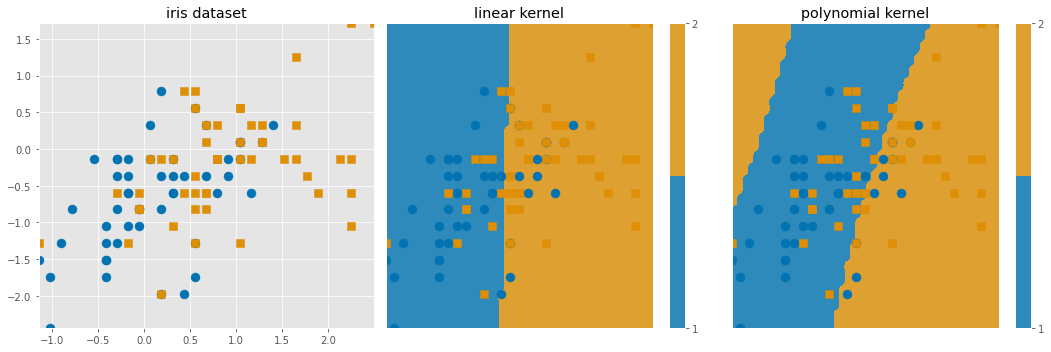
\includegraphics[width=1\textwidth]{figure 2.png}
    \caption{Visualisation des données et des frontières avec  noyau polynomial de degré 2}
    \label{fig:exemple2}
\end{figure}

\chapter{Classification des visages}

\section{Influence du paramètre de régularisation}

Dans un premier temps, nous importons, préparons et nous familiarisons avec les données.

\begin{lstlisting}[language=Python, caption=Mise en place des données]
"""
The dataset used in this example is a preprocessed excerpt
of the "Labeled Faces in the Wild", aka LFW_:

  http://vis-www.cs.umass.edu/lfw/lfw-funneled.tgz (233MB)

  _LFW: http://vis-www.cs.umass.edu/lfw/
"""

# Download the data and unzip; then load it as numpy arrays
lfw_people = fetch_lfw_people(min_faces_per_person=70, resize=0.4,
                              color=True, funneled=False, slice_=None,
                              download_if_missing=True)

# introspect the images arrays to find the shapes (for plotting)
images = lfw_people.images
n_samples, h, w, n_colors = images.shape

# the label to predict is the id of the person
target_names = lfw_people.target_names.tolist()

# Pick a pair to classify
names = ['Tony Blair', 'Colin Powell']

idx0 = (lfw_people.target == target_names.index(names[0]))
idx1 = (lfw_people.target == target_names.index(names[1]))
images = np.r_[images[idx0], images[idx1]]
n_samples = images.shape[0]
y = np.r_[np.zeros(np.sum(idx0)), np.ones(np.sum(idx1))].astype(int)

# plot a sample set of the data
plot_gallery(images, np.arange(12))
plt.show()

# Extract features (grayscale, mean per pixel)
X = (np.mean(images, axis=3)).reshape(n_samples, -1)

# Scale features
X -= np.mean(X, axis=0)
X /= np.std(X, axis=0)

# Split data into a half training and half test set
X_train, X_test, y_train, y_test, images_train, images_test =train_test_split(X, y, images, test_size=0.5, random_state=0)
\end{lstlisting}

Nous regardons à présent l'influence de C en le faisant varier.

\begin{lstlisting}[language=Python, caption=Programme de visualisation de l'influence de C]
print("--- Linear kernel ---")
print("Fitting the classifier to the training set")
t0 = time()

Cs = 10. ** np.arange(-5, 6)   # from 1e-5 to 1e5
scores = []
for C in Cs:
    clf = SVC(kernel='linear', C=C)
    clf.fit(X_train, y_train)
    scores.append(clf.score(X_test, y_test))

ind = np.argmax(scores)
print("Best C: {}".format(Cs[ind]))

plt.figure()
plt.plot(Cs, scores, marker="o")
plt.xlabel("Paramètre de régularisation C")
plt.ylabel("Score de test")
plt.xscale("log")
plt.title("Influence de C")
plt.tight_layout()
plt.show()
print("Best score: {}".format(np.max(scores)))
\end{lstlisting}

Ce code nous dit que la meilleure valeur de C est 0.001 et que le score associé est 0.88. Nous pouvons visualiser ce résultat sur la figure 2.1

\begin{figure}[H] % [H] = force l'image à rester ici
    \centering
    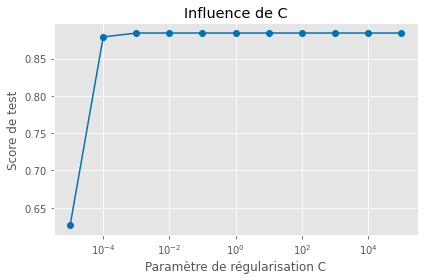
\includegraphics[width=1\textwidth]{figure 3.png}
    \caption{Score de test en fonction de la valeur du paramètre de régularisation C}
    \label{fig:exemple3}
\end{figure}

A présent, nous réentraînons le modèle avec la meilleure valeur de C trouvée, nous effectuons une prédiction sur les données de test.Nous prenons soin de mesurer le temps d'exécution et nous comparons la précision réelle du modèle avec le niveau de hasard.

\begin{lstlisting}[language=Python, caption=Utilisation de la meilleure valeur de C]
print("Predicting the people names on the testing set")
t0 = time()

# retrain best model
clf = SVC(kernel='linear', C=Cs[ind])
clf.fit(X_train, y_train)
y_pred = clf.predict(X_test)

print("done in %0.3fs" % (time() - t0))
# The chance level is the accuracy that will be reached when constantly predicting the majority class.
print("Chance level : %s" % max(np.mean(y), 1. - np.mean(y)))
print("Accuracy : %s" % clf.score(X_test, y_test))
\end{lstlisting}

Les résultats obtenus sont les suivants :\\
- temps d'exécution : 1.149 secondes\\
- niveau de hasard : 0.62\\
- précision réelle du modèle : 0.88\\
On constate sans surprise que le modèle est "utile" puisqu'il est plus performant que le hasard.

\section{Évaluation qualitative du modèle de prédiction et visualisation des coefficients}

Nous voulons à présent faire un test qualitatif sur la prédiction d'image et visualiser les coefficients appris par le modèle.

\begin{lstlisting}[language=Python, caption=Test de prédiction et visualisation des coefficients]
# Qualitative evaluation of the predictions using matplotlib

prediction_titles = [title(y_pred[i], y_test[i], names)
                     for i in range(y_pred.shape[0])]

plot_gallery(images_test, prediction_titles)
plt.show()

# Look at the coefficients
plt.figure()
plt.imshow(np.reshape(clf.coef_, (h, w)))
plt.show()
\end{lstlisting}

On obtient dans ce cas là une prédiction 100\% juste malgré un score théorique de 88\% (figure 2.2). On peut voir sur la figure 2.3 les coefficients, c'est-à-dire les traits discriminants pour le modèle, qui lui permettent de prédire une image.

\begin{figure}[H] % [H] = force l'image à rester ici
    \centering
    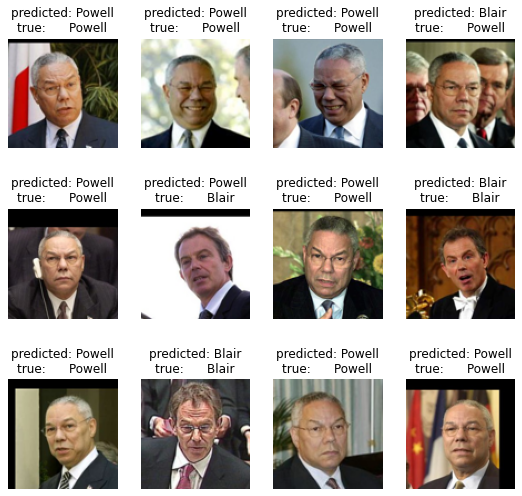
\includegraphics[width=0.5\textwidth]{figure 4.png}
    \caption{Prédiction de 12 visages}
    \label{fig:exemple4}
\end{figure}

\begin{figure}[H] % [H] = force l'image à rester ici
    \centering
    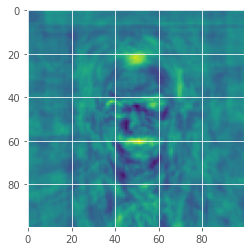
\includegraphics[width=0.5\textwidth]{figure 5.png}
    \caption{Visualisation des coefficients appris par le modèle}
    \label{fig:exemple5}
\end{figure}

\section{Influence de l'ajout de variables de nuisance}

Nous voulons tester l'influence de l'ajout de variables de nuisance. Pour cela, nous calculons le score sans variables de nuisance puis nous ajoutons 300 variables de nuisance Gaussiennes réduites.

\begin{lstlisting}[language=Python, caption=Programme de calcul de l'influence de l'ajout de variables de nuisance]
def run_svm_cv(_X, _y):
    _indices = np.random.permutation(_X.shape[0])
    _train_idx, _test_idx = _indices[:_X.shape[0] // 2], _indices[_X.shape[0] // 2:]
    _X_train, _X_test = _X[_train_idx, :], _X[_test_idx, :]
    _y_train, _y_test = _y[_train_idx], _y[_test_idx]

    _parameters = {'kernel': ['linear'], 'C': list(np.logspace(-3, 3, 5))}
    _svr = svm.SVC()
    _clf_linear = GridSearchCV(_svr, _parameters)
    _clf_linear.fit(_X_train, _y_train)

    print('Generalization score for linear kernel: %s, %s \n' %
          (_clf_linear.score(_X_train, _y_train), _clf_linear.score(_X_test, _y_test)))

print("Score sans variable de nuisance")
run_svm_cv(X, y)

print("Score avec variable de nuisance")
n_features = X.shape[1]
# On rajoute des variables de nuisance
sigma = 1
noise = sigma * np.random.randn(n_samples, 300, ) 
#with gaussian coefficients of std sigma
X_noisy = np.concatenate((X, noise), axis=1)
X_noisy = X_noisy[np.random.permutation(X.shape[0])]
run_svm_cv(X_noisy, y)
\end{lstlisting}

En généralisation, nous avons un score sans variable de nuisance de 0.94 contre un score avec variables de nuisance de 0.58. On peut donc en conclure que l'ajout de variables de nuisance fait chuter la performance du modèle.

\section{Amélioration de la prédiction à l'aide d'une réduction de dimension}

Nous effectuons une ACP afin de réduire la dimension et de voir si cela améliore comme on peut le supposer la prédiction.

\begin{lstlisting}[language=Python, caption=Prédiction avec l'utilisation de l'ACP pour réduire la dimension]
print("Score apres reduction de dimension")

n_components = 80  # jouer avec ce parametre
pca = PCA(n_components=n_components, svd_solver='randomized').fit(X_noisy)
X_pca = pca.transform(X_noisy)
run_svm_cv(X_pca, y)
\end{lstlisting}

Nous obtenons un score de 0.83 sur l'échantillon d'entraînement et de 0.52 sur l'échantillon test. Ce qui paraît anormal car une sélection de variables sachant que 300 d'entre elles sont du bruit (nous le savons puisque c'est nous qui les avons ajoutées) devrait augmenter le score de prédiction.

\section{Biais dans le prétraitement des données}

En prenant du recul sur notre travail, on peut constater qu'il y a un biais dans le prétraitement de nos données. En effet, nous effectuons la moyenne sur les canaux de couleurs, pour ne garder que l'illumination moyenne par pixel, ce qui engendre une perte d'information. 

\begin{lstlisting}[language=Python, caption=Hypothèse d'une commande source de perte d'information]
X = (np.mean(images, axis=3)).reshape(n_samples, -1)
\end{lstlisting}

\chapter{Code complet}

\begin{lstlisting}[language=Python, caption=Code python complet]
#%%
import numpy as np
import matplotlib.pyplot as plt
from sklearn.svm import SVC

from svm_source import *
from sklearn import svm
from sklearn import datasets
from sklearn.utils import shuffle
from sklearn.preprocessing import StandardScaler
from sklearn.model_selection import train_test_split, GridSearchCV
from sklearn.datasets import fetch_lfw_people
from sklearn.decomposition import PCA
from time import time

scaler = StandardScaler()

import warnings
warnings.filterwarnings("ignore")

plt.style.use('ggplot')

#%%
####################################################################
#               Toy dataset : 2 gaussians
####################################################################

n1 = 200
n2 = 200
mu1 = [1., 1.]
mu2 = [-1./2, -1./2]
sigma1 = [0.9, 0.9]
sigma2 = [0.9, 0.9]
X1, y1 = rand_bi_gauss(n1, n2, mu1, mu2, sigma1, sigma2)

plt.show()
plt.close("all")
plt.ion()
plt.figure(1, figsize=(15, 5))
plt.title('First data set')
plot_2d(X1, y1)

X_train = X1[::2]
Y_train = y1[::2].astype(int)
X_test = X1[1::2]
Y_test = y1[1::2].astype(int)

# fit the model with linear kernel
clf = SVC(kernel='linear')
clf.fit(X_train, Y_train)

# predict labels for the test data base
y_pred = clf.predict(X_test)

# check your score
score = clf.score(X_test, Y_test)
print('Score : %s' % score)

# display the frontiere
def f(xx):
    """Classifier: needed to avoid warning due to shape issues"""
    return clf.predict(xx.reshape(1, -1))

plt.figure()
frontiere(f, X_train, Y_train, w=None, step=50, alpha_choice=1)

# Same procedure but with a grid search
parameters = {'kernel': ['linear'], 'C': list(np.linspace(0.001, 3, 21))}
clf2 = SVC()
clf_grid = GridSearchCV(clf2, parameters, n_jobs=-1)
clf_grid.fit(X_train, Y_train)

# check your score
print(clf_grid.best_params_)
print('Score : %s' % clf_grid.score(X_test, Y_test))

def f_grid(xx):
    """Classifier: needed to avoid warning due to shape issues"""
    return clf_grid.predict(xx.reshape(1, -1))

# display the frontiere
plt.figure()
frontiere(f_grid, X_train, Y_train, w=None, step=50, alpha_choice=1)

#%%
####################################################################
#               Iris Dataset
####################################################################

iris = datasets.load_iris()
X = iris.data
X = scaler.fit_transform(X)
y = iris.target
X = X[y != 0, :2]
y = y[y != 0]

# split train test (say 25% for the test)
# Split train/test
X_train, X_test, y_train, y_test = train_test_split(X, y, test_size=0.25, random_state=42, shuffle=True)

####################################################################
# fit the model with linear vs polynomial kernel
####################################################################

#%%
# Q1 Linear kernel

# fit the model and select the best hyperparameter C
parameters = {'kernel': ['linear'], 'C': list(np.logspace(-3, 3, 200))}
clf_linear = GridSearchCV(SVC(), parameters, n_jobs=-1)
clf_linear.fit(X_train, y_train)

# compute the score
print(clf_linear.best_params_)
print('Generalization score for linear kernel: %s, %s' %
      (clf_linear.score(X_train, y_train),
       clf_linear.score(X_test, y_test)))

#%%
# Q2 polynomial kernel
Cs = list(np.logspace(-3, 3, 5))
gammas = 10. ** np.arange(1, 2)
degrees = np.r_[1, 2, 3]

# fit the model and select the best set of hyperparameters
parameters = {'kernel': ['poly'], 'C': Cs, 'gamma': gammas, 'degree': degrees}

clf_poly = GridSearchCV(SVC(), parameters, n_jobs=-1)
clf_poly.fit(X_train, y_train)

print(clf_poly.best_params_)
print('Generalization score for polynomial kernel: %s, %s' %
      (clf_poly.score(X_train, y_train),
       clf_poly.score(X_test, y_test)))

#sans le degre 1
Cs = list(np.logspace(-3, 3, 5))
gammas = 10. ** np.arange(1, 2)
degrees = np.r_[2, 3]

# fit the model and select the best set of hyperparameters
parameters = {'kernel': ['poly'], 'C': Cs, 'gamma': gammas, 'degree': degrees}

clf_poly2 = GridSearchCV(SVC(), parameters, n_jobs=-1)
clf_poly2.fit(X_train, y_train)

print(clf_poly2.best_params_)
print('Generalization score for polynomial kernel: %s, %s' %
      (clf_poly2.score(X_train, y_train),
       clf_poly2.score(X_test, y_test)))


#%%
# display your results using frontiere (svm_source.py)

def f_linear(xx):
    return clf_linear.predict(xx.reshape(1, -1))

def f_poly(xx):
    return clf_poly.predict(xx.reshape(1, -1))

plt.ion()
plt.figure(figsize=(15, 5))
plt.subplot(131)
plot_2d(X, y)
plt.title("iris dataset")

plt.subplot(132)
frontiere(f_linear, X, y)
plt.title("linear kernel")

plt.subplot(133)
frontiere(f_poly, X, y)
plt.title("polynomial kernel")

plt.tight_layout()
plt.draw()

def f_poly2(xx):
    return clf_poly2.predict(xx.reshape(1, -1))

plt.ion()
plt.figure(figsize=(15, 5))
plt.subplot(131)
plot_2d(X, y)
plt.title("iris dataset")

plt.subplot(132)
frontiere(f_linear, X, y)
plt.title("linear kernel")

plt.subplot(133)
frontiere(f_poly2, X, y)
plt.title("polynomial kernel")

plt.tight_layout()
plt.draw()

#%%
####################################################################
#               Face Recognition Task
####################################################################
"""
The dataset used in this example is a preprocessed excerpt
of the "Labeled Faces in the Wild", aka LFW_:

  http://vis-www.cs.umass.edu/lfw/lfw-funneled.tgz (233MB)

  _LFW: http://vis-www.cs.umass.edu/lfw/
"""

####################################################################
# Download the data and unzip; then load it as numpy arrays
lfw_people = fetch_lfw_people(min_faces_per_person=70, resize=0.4,
                              color=True, funneled=False, slice_=None,
                              download_if_missing=True)

# introspect the images arrays to find the shapes (for plotting)
images = lfw_people.images
n_samples, h, w, n_colors = images.shape

# the label to predict is the id of the person
target_names = lfw_people.target_names.tolist()

####################################################################
# Pick a pair to classify
names = ['Tony Blair', 'Colin Powell']

idx0 = (lfw_people.target == target_names.index(names[0]))
idx1 = (lfw_people.target == target_names.index(names[1]))
images = np.r_[images[idx0], images[idx1]]
n_samples = images.shape[0]
y = np.r_[np.zeros(np.sum(idx0)), np.ones(np.sum(idx1))].astype(int)

# plot a sample set of the data
plot_gallery(images, np.arange(12))
plt.show()

####################################################################
# Extract features (grayscale, mean per pixel)
X = (np.mean(images, axis=3)).reshape(n_samples, -1)

# Scale features
X -= np.mean(X, axis=0)
X /= np.std(X, axis=0)

####################################################################
# Split data into a half training and half test set
X_train, X_test, y_train, y_test, images_train, images_test =train_test_split(X, y, images, test_size=0.5, random_state=0)

####################################################################

# Q4 Influence of regularization parameter C
print("--- Linear kernel ---")
print("Fitting the classifier to the training set")
t0 = time()

Cs = 10. ** np.arange(-5, 6)   # from 1e-5 to 1e5
scores = []
for C in Cs:
    clf = SVC(kernel='linear', C=C)
    clf.fit(X_train, y_train)
    scores.append(clf.score(X_test, y_test))

ind = np.argmax(scores)
print("Best C: {}".format(Cs[ind]))

plt.figure()
plt.plot(Cs, scores, marker="o")
plt.xlabel("Paramètre de régularisation C")
plt.ylabel("Score de test")
plt.xscale("log")
plt.title("Influence de C")
plt.tight_layout()
plt.show()
print("Best score: {}".format(np.max(scores)))

print("Predicting the people names on the testing set")
t0 = time()

# retrain best model
clf = SVC(kernel='linear', C=Cs[ind])
clf.fit(X_train, y_train)
y_pred = clf.predict(X_test)

print("done in %0.3fs" % (time() - t0))
# The chance level is the accuracy that will be reached when constantly predicting the majority class.
print("Chance level : %s" % max(np.mean(y), 1. - np.mean(y)))
print("Accuracy : %s" % clf.score(X_test, y_test))

####################################################################

#%%
####################################################################
# Qualitative evaluation of the predictions using matplotlib

prediction_titles = [title(y_pred[i], y_test[i], names)
                     for i in range(y_pred.shape[0])]

plot_gallery(images_test, prediction_titles)
plt.show()

####################################################################
# Look at the coefficients
plt.figure()
plt.imshow(np.reshape(clf.coef_, (h, w)))
plt.show()


#%%
# Q5

def run_svm_cv(_X, _y):
    _indices = np.random.permutation(_X.shape[0])
    _train_idx, _test_idx = _indices[:_X.shape[0] // 2], _indices[_X.shape[0] // 2:]
    _X_train, _X_test = _X[_train_idx, :], _X[_test_idx, :]
    _y_train, _y_test = _y[_train_idx], _y[_test_idx]

    _parameters = {'kernel': ['linear'], 'C': list(np.logspace(-3, 3, 5))}
    _svr = svm.SVC()
    _clf_linear = GridSearchCV(_svr, _parameters)
    _clf_linear.fit(_X_train, _y_train)

    print('Generalization score for linear kernel: %s, %s \n' %
          (_clf_linear.score(_X_train, _y_train), _clf_linear.score(_X_test, _y_test)))

print("Score sans variable de nuisance")
run_svm_cv(X, y)

print("Score avec variable de nuisance")
n_features = X.shape[1]
# On rajoute des variables de nuisances
sigma = 1
noise = sigma * np.random.randn(n_samples, 300, ) 
#with gaussian coefficients of std sigma
X_noisy = np.concatenate((X, noise), axis=1)
X_noisy = X_noisy[np.random.permutation(X.shape[0])]
run_svm_cv(X_noisy, y)

#%%
# Q6
print("Score apres reduction de dimension")

n_components = 100  # jouer avec ce parametre
pca = PCA(n_components=n_components, svd_solver='randomized').fit(X_noisy)
X_pca = pca.transform(X_noisy)
run_svm_cv(X_pca, y)

\end{lstlisting}

\end{document}


